%TeX root = ../main.tex
\chapter{Holomorphic Fourier Transforms}

\section{Motivation and Basic Results}
In last chapter we explored the Fourier transforms of functions in $\R$. Frequently the fourier transform of functions in $\R$ can be extended to a holomorphic function in certain regions. For example say $f(x) = e^{-|x|}$, then $\hatf(t) = \frac{1}{1+(2\pi t)^2}$. 
Since, 
\begin{align*}
  \hatf(t) = \int_\R e^{-|x|}e^{-2 \pi itx} \ dx &= \int_{-\infty}^0 e^{x(1-2\pi it)} \ dx + \int_0^{\infty} e^{-x(1+2\pi it)} \ dx \\
  & = \left[ \frac{e^{x(1-2\pi it)}}{1-2\pi it}\right]_{-\infty}^0 - \left[ \frac{e^{-x(1+2\pi it)}}{1+2\pi it}\right]^{\infty}_0 \\
  & = \frac{1}{1-2\pi it} + \frac{1}{1+2\pi it} \\
  &= \frac{1}{1+(2\pi t)^2}
\end{align*}
Clearly $w(z) = \frac{1}{1+(2\pi z)^2}$ is a holomorphic extension of $\hatf$ into the regions of the complex plane without the points $z=\pm \frac{i}{2\pi}$.

We will study two classes of functions which can be extended in this manner. The first class of such functions is $$f(z) = \int_0^\infty F(t)e^{2\pi i tz}\ dt$$
where $z\in \Pi^+ = \{z\in \C \ | \Im(z) > 0 \}$ and $F \in L^2(\R)$ is a function which vanishes on $(-\infty, 0)$. The second class of functions will be $$f(z) = \int_{-A}^A F(t)e^{2\pi i t z} \ dt$$
where $0<A<\infty$ and $F \in L^2(-A, A)$. We'll now prove some important results regarding these two classes of functions

\begin{proposition}
  \label{prop:fourier_transform_in_upper_half_plane}
  Let $F\in L^2(\R)$ such that $F$ vanishes at $(-\infty , 0)$. Then $f : \Pi^+ \to \C$ defined as, $$f(z) = \int_0^\infty F(t) e^{2\pi itz} \ dt$$
  is holomorphic in the upper half plane, i.e $f \in H(\Pi^+)$. Moreover $f$ restricted to horizontal lines in $\Pi^+$ is bounded in the  $L^2$ norm and the bound is independent of the horizontal line. That is if $z = x+iy$, then $$\sup_{0<y<\infty}\int_{-\infty}^\infty \left|f(x + iy)\right|^2 \ dx = \int_0^\infty |F(t)|^2 \ dt < \infty$$
\end{proposition}
\begin{proof}
  Let $z \in \Pi^+$. Then there exists a $\delta$ such that $0< \delta < \Im(z)$. Since $\Pi^+$ is open, there exists a sequence $z_n$ in $\Pi^+$ such that $\delta < \Im(z_n)$, and  $z_n \to z$. Also 
  \begin{align*}
    \left|e^{2 \pi itz_n} - e^{2\pi itz}\right|^2 &= \left|\left(e^{2\pi it z_n} - e^{2\pi itz}\right)^2\right| \\ 
    &= \left| e^{4\pi itz_n} + e^{4\pi itz} - 2e^{2\pi it(z+z_n)} \right| \\
    &\le \left|e^{4\pi itz_n}\right| + \left|e^{4\pi itz}\right| + 2\left|e^{2\pi it(z_n + z)}\right| \\
    &= e^{-4\pi t \Im(z_n)} + e^{-4 \pi t \Im(z)} + 2e^{-2\pi t \Im(z_n - z)} \\
    &\le e^{-4\pi t \delta} + e^{-4\pi t \delta} + 2e^{-4 \pi t\delta} \\
    &=4e^{-4\pi t \delta}
  \end{align*}
  Now since $$\int_0^\infty 4e^{-4\pi t\delta} \ dt = \frac{4}{2\pi \delta}$$
  the integrad is $L^1$ in $(0, \infty)$ and therefore by dominated convergence theorem, $$\lim_{n \to \infty} \int_0^\infty \left|e^{2\pi itz_n} - e^{2\pi itz}\right|^2 \ dt = 0$$
  Now therefore if $w \in \Pi^+$ and $w_n \to w$, then 
  \begin{align*}
    f(w_n) - f(w) &= \int_0^\infty F(t)(e^{2\pi it w_n} - e^{2\pi i tw}) \ dt \\
    & \le \|F\|_2 \|e^{2\pi itw_n} - e^{2\pi itw}\|_2
  \end{align*}
  By assumption $\|F\|_2$ is a finite quantity and from above result $\|e^{2\pi itw_n} - e^{2\pi itw}\|_2 \to 0$ as $w_n \to w$. Therefore $f(w_n) \to f(w)$. Since our choice of $w$ was arbitary, this implies that $f$ is continuous everywhere in $\Pi^+$. Also if $\gamma$ is any triangle in $\Pi^+$, then $\gamma$ can be parametrized by $s \in [a, b]$ as $\gamma(s) = x(s) + iy(s)$, where $y(s) >0$ since $\gamma \in \Pi^+$. Now let $M = \sup_{s \in [a,b]} |\gamma^{'}(s)|$ (here we take only differentiable points in $\gamma$ for supremum, since the non-differentiable points will be measure zero and adds nothing to the integral). Also since $\gamma \in \Pi^+$, there exist an $m >0$ such that $y(s) > m$ for all $s$. Then we get that
  \begin{align*}
    \int_{\gamma}\int_{0}^{\infty}|F(t)e^{itz}|\,dt\,d|z|&=
    \int_a^b\int_{0}^{\infty}|F(t)|e^{-ty(s)}\,dt\,|\gamma'(s)|\,ds\\
    &\leq M\int_a^b\int_{0}^{\infty}|F(t)|e^{-mt}\,dt\,ds\\
    &=M(b-a)\int_{0}^{\infty}|F(t)|e^{-mt}\,dt\\
    &\leq M(b-a)\|F\|_{L^2((0,\infty))}\cdot\left(\int_{0}^{\infty}(e^{-mt})^2\,dt\right)^{1/2}
  \end{align*}
  Therfore by Fubini's Theorem we can change the order of integration and we get, 
  \begin{align*}
    \int_\gamma f(z)\ dz &= \int_\gamma \int_0^\infty F(t) e^{2\pi i t z} \ dt \ dz \\
    & = \int_0^\infty F(t) \int_\gamma e^{2\pi itz} \ dz \ dt \\
    & = \int_0^\infty F(t) \cdot 0 \ dt \\
    & = 0
  \end{align*}
  Then by Morera's theorem, $f$ is holomorphic everywhere in the upper half plane.

  Now consider $z=x+iy$, then $f$ can be written as $$f(x+iy) = \int_0^\infty F(t)e^{2\pi i t (x+iy)}\ dt = \int_0^\infty F(t)e^{-2\pi ty}e^{2\pi i tx} \ dt$$ 
  Now for a fixed $y \in \R$, consider $g_y(t) = F(t)e^{-2\pi ty}$. Then from above equation $f(x+iy) = \widehat{g_y}(x)$. By Holder's inequality we get that 
  \begin{align*}
    \int_0^\infty |g_y(t)| \ dt &= \int_0^\infty \left|F(t)e^{-2\pi ty}\right| \ dt \\
    &\le \left(\int_0^\infty \left|F(t)\right|^2 \ dt \right)^{\frac{1}{2}} \left(\int_0^\infty e^{-4\pi ity} \ dt \right)^{\frac{1}{2}}
  \end{align*}
  where both of the integrals are finite. Therefore $g_y \in L^1(0, \infty)$. Again since $0<e^{-x}\le1$ when $0\le x<\infty$, we know that $$\int_0^\infty |g_y(t)|^2 \ dt = \int_0^\infty \left|F(t)\right|^2 \left| e^{-2\pi ty} \right|^2 \ dt \le \int_0^\infty \left|F(t)\right|^2 \ dt$$
  which is again finite. Therefore $g\in L^2(0, \infty)$. Therefore by Plancherel's theorem (refer theorem \ref{thm:Plancherel's_theorem}) on $g_y$ we get that, $$\int_{-\infty}^{\infty}\left|f(x+iy)\right|^2 \ dx = \int_{-\infty}^{\infty} \left|\widehat{g_y}(x)\right|^2 \ dx= \int_{-\infty}^{\infty} \left|g_y(t)\right|^2 \ dt = \int_0^\infty \left|g_y(t)\right|^2 \ dt $$
Note that the change in limit in the last integral is because $g_y(t) = 0$ when $t < 0$. But from last inequality $$\int_0^\infty \left|g_y(t)\right|^2 \ dt \le \int_0^\infty \left|F(t)\right|^2 \ dt$$
  which is finite since $F \in L^2(0, \infty)$, and independent of $y$. Therefore $$\sup_{0<y<\infty} \int_{-\infty}^\infty \left|f(x+iy)\right|^2 \ dx \le \int_0^\infty \left|F(t)\right|^2 \ dt $$
  Moreover by Lebesgue dominated convergence theorem we get that $$\lim_{y \searrow 0} \int_0^\infty |g_y(t)|^2 \ dt = \int_0^\infty |F(t)|^2 \ dt$$
  Therefore $$\sup_{0<y<\infty} \int_{-\infty}^\infty \left|f(x+iy)\right|^2 \ dx = \int_0^\infty \left|F(t)\right|^2 \ dt $$
\end{proof}

\begin{proposition}
  Let $0<A<\infty$ and $F \in L^2(-A, A)$. Then $f:\C \to \C$ defined as $$f(z) = \int_{-A}^A F(z)e^{2\pi itz} \ dt$$
  is an entire function which satisfy $$|f(z)| \le Ce^{2 \pi A|z|}$$
  for some constant $C$ and $f$ when restricted to horizontal lines is bounded in the $L^2$ norm. That is if $f(z)$ is written as $f(x+iy)$ then  $$\int_{-\infty}^{\infty} |f(x+iy)|^2 \ dx < \infty$$
\end{proposition}
\begin{proof}
  Like in proof of the above theorem for $z\in \C$ we write $z = x+iy$. Then $$f(x+iy) = \int_{-A}^A F(t) e^{2\pi it(x+iy)} \ dt = \int_{-A}^A F(t)e^{-2\pi ty}e^{2\pi itx} \ dt$$
  Therefore since $|e^{2\pi it x}| = 1$, $$\left|f(x+iy)\right| \le \int_{-A}^A \left|F(t)\right| e^{-2\pi ty} \ dt \le e^{2\pi A|y|} \int_{-A}^A \left|F(t)\right| \ dt $$
  We know that $F \in L^2(-A, A)$. But since $(-A, A)$ under Lebesgue measure is a finite measure space, $f \in L^1(-A, A)$. And therefore the last integral above is finite. Let's call it $C$. Also since $e^{\Im(z)} \le e^z$, it follows that $$\left|f(z) \right| \le Ce^{2\pi A |z|}$$

  Now consider points $z \in \C$. Then for $\delta \in \C$,
  \begin{align*}
    f(z+\delta) - f(z) &= \int_{-A}^A F(t)\left(e^{it(z+\delta)} - e^{itz}\right) \ dt \\
    &\le \left(\int_{-A}^A \left|F(t)\right|^2\ dt \right)^{\frac{1}{2}} \left(\int_{-A}^A \left|e^{it(z+\delta)}-e^{itz}\right|^2 \ dt \right)^{\frac{1}{2}}
  \end{align*}
  Now the first integral is finite since $F\in L^2(-A, A)$. Again since $e^{itz}$ is a continuous function in a finite measure space it is in $L^2(-A, A)$ and by a change of variable $r = At$, a we can use proposition \ref{prop:L2_functions_are_continuous_in_L2_norm} and conclude that the second integral converge to zero as $\delta \to 0$. Therefore $f$ is continuous in the whole of $\C$. 

  Moreover if $\gamma$ is any closed path in $\C$, and $\Omega$ is the interior of the space enclosed by $\gamma$, then $(-A, A)\times\Omega$ is a finite measure space. Therefore by Fubini's Theorem we change of order of integration and $$\int_\gamma f(z) \ dz = \int_\gamma \int_{-A}^A F(t)e^{2\pi itz} \ dt \ dz = \int_{-A}^A F(t) \int_\gamma e^{2\pi itz} \ dz \ dt = \int_{-A}^A F(t)\cdot 0 \ dt = 0$$
  since $e^{2\pi itz}$ is entire. Then by Morera's theorem, $f$ is entire.

  We'll now prove that restrictioins of $f$ in to horizontal lines are bounded in the $L^2$ norm. For this let $$g_y(t) = F(t)e^{-2\pi ty}$$
  Then from the first equation in the proof, we get that $$f(x+iy) = \int_{-A}^A g_y(t) e^{2\pi itx} \ dt$$
which implies that $f$ restricted to horizontal lines is the inverse Fourier transform of $g_y$ in the domain $(-A, A)$. Also by the definition of $g_y$, $$\int_{-A}^A \left|g_y(t)\right|^2 \ dt = \int_{-A}^A \left|F(t)\right|^2 e^{-4\pi t y} \ dt \le e^{\left|4\pi Ay\right|}\int_{-A}^A \left|F(t)\right|^2 \ dt$$
  Since by assumption $F \in L^2(-A, A)$, $g_y \in L^2(-A, A)$. Since $(-A, A)$ is a finite measure space $g_y \in L^1(-A, A)$. Now using Plancherel's theorem (\autoref{thm:Plancherel's_theorem}), we get that $$\int_{-\infty}^\infty |f(x+iy)|^2 \ dx = \int_{-\infty}^\infty |\widehat{g_y}(x)|^2 \ dx = \int_{-A}^A |g_y(t)|^2 \ dt $$
  Therefore, $f$ restricted to horizontal lines is bounded in $L^2$.
\end{proof}

\section{Paley Wiener Theorems}
What is interesting is that the converse of the above two results is also true. These are known as the classical Paley Wiener theorems. With the help of these we can extend the definition of Fourier transforms to holomorphic functions in the upper half plane and entire functions of exponential type (functions where $|f(z)| \le Ce^{2\pi A |z|}$).

\begin{theorem}[Paley Wiener Theorem]
  \label{thm:paley_wiener_in_upper_half_plane}
  Let $f \in H(\Pi^+)$ and $$\sup_{0<y<\infty} \frac{1}{2\pi} \int_\R |f(x+iy)|^2 \ dx = C < \infty$$
  Then there exists an $F \in L^2(0, \infty)$ such that for $z \in \Pi^+$, $$f(z) = \int_0^\infty F(t)e^{2\pi itz} \ dt$$
  and 
  $$\int_0^\infty |F(t)|^2 \ dt = C $$
\end{theorem}
\begin{note}
  Let's analyse this intuitively. Rewriting the second equation in the theorem, we see that $$f(x+iy) = e^{-2\pi ty}\int_0^\infty F(t) e^{2\pi itx} \ dt $$
  which implies
  $$\int_0^\infty F(t) e^{2\pi itx} \ dt = e^{2\pi t y}f(x+iy)$$
  From this we see that the required function $F$ is the inverse transform of $f(x+iy)e^{2\pi ty}$ along the horizontal line $\Im(z) = y$
  Therefore a good candidate is $$F(t) = \int_\R f(x+iy)e^{2\pi ty}e^{-2\pi itx} \ dx = \int_{\Im(z) = y} f(z)e^{-2\pi itz} \ dz$$
  Here the left hand side of the equation seems to be depending on only $t$, while the left hand side seems to depend on $y$. So we will have that the value fo $F(t)$ is independent of $y$, i.e $F(t)$ will depend only on the choice of the function $f$ and not the horizontal lines in which $f$ is evaluated.
  \end{note}
\begin{proof}
  % Since we'll be working with horizontal lines, let's fix the notation that $f_y(x) = f(x+iy)$. Since $f_y \in L^2(\R)$ for all $y>0$, by Plancherel's Theorem (\autoref{thm:Plancherel's_theorem}) $\widehat{f_y}$ exists and is in $L^2(\R)$. We'll fix $F(t) = e^{2\pi t}\widehat{f_1}(t)$. 
  % Then as we discussed above we'll need to prove that for two different horizontal lines $\Im(z) = y_1$ and $\Im(z) = y_2$, $e^{2\pi ity_1}\widehat{f_{y_1}} = e^{2\pi ity_2}\widehat{f_{y_2}}$
  %
  We'll first try to prove that our choice of $F$ from above is independent of $y$, i.e the horizontal lines.
  Fix $y$, where $0<y< \infty$ and for each $\alpha >0$, consider the rectangular path $\Gamma_\alpha$ with vertices at $\pm \alpha + i$ and $\pm \alpha + iy$. Then since $\Gamma_\alpha \subset \Pi^+$ and for a fixed $t \in \R$ \ $f, e^{-2\pi itz} \in H(\Pi^+)$, 
  \begin{equation}
    \label{eqn:eqn_holomorphic_stuff}
    \int_{\Gamma_\alpha} f(z)e^{-2\pi itz} \ dz = 0
  \end{equation}
  For $\beta \in \R$ and $I= [1, y]$ if $1<y$ (otherwise let $I=[y, 1]$) let $$\Phi(\beta) = \int_I f(\beta + iu)e^{-2\pi it(\beta+iu)} \ du$$

  
  Now by Cauchy Schwarz inequality, we get that
  \begin{equation}
    |\Phi(\beta)|^2 \le \left(\int_I |f(\beta+iu)|^2 \ du \right)\left(\int_I e^{4\pi \beta u} \ dt \right)
    \label{eqn:lets_see_abtthis_eqn}
  \end{equation}
  where the last integral is finite being the integral of a continuous function in a compact interval. And as for the first interal, since the space is $\sigma$-finite, by Fubini-Tonelli theorem
  \begin{align*}
    \int_\R \int_I |f(\beta + iu)|^2 \ du \ d\beta &= \int_I \int_\R |f(\beta + iu)|^2 \ d\beta \ du \\
    & \le C|y-1| 
  \end{align*}
  where $C$ is the constant in the assumption that restriction of $f$ into horizontal lines are uniformly bounded in $L^2(\R)$.

  Hence $\int_I |f(\beta+iu)|^2 \ du$ is integrable and therefore there exist a sequence $\{\alpha_j\}$ such that $\alpha_j \to \infty$ as $j \to \infty$ and
  \begin{equation}
  \label{eqn:some_blah_blah_blah}
  \lim_{j \to \infty} \int_I f(\alpha_j + iu) \ du = \lim_{j \to \infty} \int_I f(-\alpha_j + iu) \ du = 0
  \end{equation}
 
  Therefore $\Phi(\alpha_j) \to 0, \Phi(-\alpha_j) \to 0$ as $j \to \infty$.
 
  \begin{figure}
    \centering
    \begin{tikzpicture}
      % Draw the x-axis and y-axis
      \draw[->] (-5,0) -- (5,0) node[below right] {$\Re(z)$};
      \draw[->] (0,-1) -- (0,4) node[above left] {$\Im(z)$};
 
      % Draw the rectangle with one edge on the line y=1
      \draw[thick] (-2,1) rectangle (2,3);
      \draw[dotted] (-3,1) rectangle (3,3);
      \fill[cyan, opacity=0.3] (-2,1) -- (-2, 3) -- (2, 3) -- (2, 1) -- cycle;
      \draw[dotted] (-4,1) rectangle (4,3);

      \node[left] at (0, 2) {$\Gamma_{\alpha_j}$};
      \node[above right] at (0, 1) {$1$};
      \node[above right] at (0, 3) {$y$};
      \node[circle, fill, inner sep=1pt, label=below:$\alpha_j$] at (2, 0) {};
      \node[circle, fill, inner sep=1pt, label=below:$\alpha_{j+1}$] at (3, 0) {};
      \node[circle, fill, inner sep=1pt, label=below:$\alpha_{j+2}$] at (4, 0) {};
      \node[circle, fill, inner sep=1pt, label=below:$-\alpha_j$] at (-2, 0) {};
      \node[circle, fill, inner sep=1pt, label=below:$-\alpha_{j+1}$] at (-3, 0) {};
      \node[circle, fill, inner sep=1pt, label=below:$-\alpha_{j+2}$] at (-4, 0) {};
      \node[left] at (-2, 2) {\rotatebox{90}{$\xrightarrow{\Phi(-\alpha_j)}$}};
      \node[left] at (2, 2) {\rotatebox{90}{$\xrightarrow{\Phi(\alpha_j)}$}};
    \end{tikzpicture}
    \caption{Indicative diagram shows the domains of integration}
  \end{figure}

  Also by \autoref{eqn:eqn_holomorphic_stuff},
  \begin{equation*}
    \begin{split}
      \int_{-\alpha_j+i}^{-\alpha_j +yi} f(z)e^{-2\pi it z} \ dz + \int_{-\alpha_j+yi}^{\alpha_j +yi} f(z)e^{-2\pi it z} \ dz &= \int_{-\alpha_j+i}^{\alpha_j +i} f(z)e^{-2\pi it z} \ dz \\
      &+ \int_{\alpha_j+i}^{\alpha_j +yi} f(z)e^{-2\pi it z} \ dz
    \end{split}
  \end{equation*}
  Now taking limit as $j \to \infty$ on both sides and by \autoref{eqn:some_blah_blah_blah}, we get that $$\lim_{j\to \infty} \int_{-\alpha_j+yi}^{\alpha_j +yi} f(z)e^{-2\pi it z} \ dz = \lim_{j \to \infty} \int_{-\alpha_j +i}^{\alpha_j +i} f(z)e^{-2\pi it z}$$
  Therefore,
  $$\int_\R f(x+iy)e^{-2\pi i t(x+iy)} \ dx = \int_\R f(x+i)e^{-2\pi it(x+i)} \ dx$$
  Now for a fixed $y>0$ and $f_y(x) = f(x+iy)$, take $F(t) = e^{2\pi ty}\widehat{f}(t)$, where $\widehat{f_y}$, is the Fourier transform of $f_y$. Then by previous equality we get that, 
  \begin{align*}
    F(t) &= e^{2\pi ty} \widehat{f_y}(t)\\
          &= e^{2\pi ty}\int_\R f(x+iy) e^{-2\pi itx} \ dx \\
          &= \int_\R f(x+iy)e^{-2\pi t(x+iy)} \ dx \\
          &= \int_\R f(x+i)e^{-2\pi t(x+i)} \ dx \\
          &= e^{2\pi t}\int_\R f(x+i) e^{-2\pi itx} \ dx \\
          &= e^{2\pi t} \widehat{f_1}(t) \\
  \end{align*}
  Thus we see that $F(t)$ is independent of our choice of horizontal line.
 
  Now by Plancherel's theorem (\autoref{thm:Plancherel's_theorem}), $\|f_y\|_2 = \|\widehat{f_y}\|_2$, and for every $y>0$
  $$\int_\R e^{-4 \pi t y} |F(t)|^2 \ dt = \int_\R |\widehat{f_y}(t)|^2 \ dt = \int_\R |f_y(t)|^2 \ dt \le C$$
  where $C$ is the constant in the assumption of the theorem.
  Now by monotone convergence theorem, as $y\to \infty$, this shows that $F(t) =0$ almost everywhere in $(-\infty, 0)$. Again as $y \to 0$, we get that $$\int_0^\infty |F(t)|^2 \ dt \le C$$

  Again since $\widehat{f_y}(t) = F(t)e^{-2\pi ty}$ and $F(t) = 0$ almost everywhere in $(-\infty, 0)$, by Cauchy Schwarz inequality, we get
  $$\int_\R |\widehat{f_y}(t)| \ dt = \int_{0}^\infty F(t) e^{-2\pi ty} \ dy < \infty$$
  Hence $\widehat{f_y} \in L^1(\R)$ and by Fourier inversion
  $$f(z) = f_y(x) = \int_\R \widehat{f_y}(t) e^{2\pi it x}\ dt = \int_0^\infty F(t)e^{2\pi it(x+iy)} \ dt = \int_{0}^\infty F(t)e^{2\pi itz} \ dz$$
  And from \autoref{prop:fourier_transform_in_upper_half_plane} it follows that $$\int_0^\infty |F(t)|^2 \ dt = C$$
\end{proof}

\begin{theorem}[Paley Wiener Theorem]
  \label{thm:paley_wiener_2}
  Suppose $A$ and $C$ are positive constants and $f$ is an entire function such that for all $z \in \C$, $$|f(z)| \le Ce^{2\pi A |z|}$$
  and restriction of $f$ into horizontal lines is in $L^2$, i.e $$\int_{-\infty}^\infty |f(x +iy)|^2 \ dx < \infty$$
  Then there exists an $F \in L^2(-A, A)$ such that for all $z\in \C$, $$f(z) = \int_{-A}^A F(t)e^{2 \pi it z} \ dt $$
\end{theorem}
\begin{proof}
  Before we start analysing on $f$, we'll define $f_\epsilon(x) = f(x)e^{-2\pi \epsilon |x|}$

  \textbf{Step 1}: For each $\alpha \in \R$ define $\Gamma_\alpha$ to be the ray, $$\Gamma_\alpha(s) = se^{i\alpha}$$
  where $0\le s <\infty$ and $$\Pi_\alpha = \{w\ | \ \Re(we^{i\alpha}) > A\}$$

   \begin{figure}[h]
     \centering
      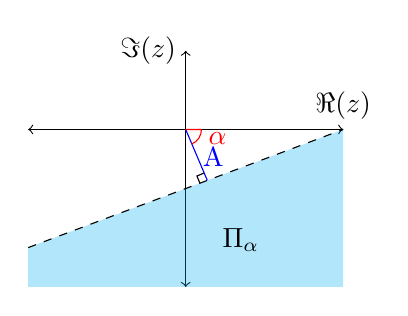
\begin{tikzpicture}
        % Draw axes
        \draw[<->] (-2,0) -- (2,0) node[above] {$\Re(z)$};
        \draw[<->] (0,-2) -- (0,1) node[left] {$\Im(z)$};
        \fill[cyan,opacity=0.3] (-2,-1.5) -- (-2, -2) -- (2,-2) -- (2, 0) -- cycle;
        \draw[dashed] (-2, -1.5) -- (2, 0);
        % Draw line
        \draw[blue,rotate=-67] (0,0) -- (0.7,0);
        \node at (0.35, -0.35) {\color{blue}{A}};
        \node at (0.7, -1.4) {$\Pi_\alpha$};
        \draw[red] (0, 0) -- (0:0.2) arc (0:-68:0.2) node[midway, right] {\color{red}{$\alpha$}};
        \draw[rotate=-67] (0.6, 0) -- (0.6, -0.1) -- (0.7, -0.1);
      \end{tikzpicture}
      \caption{Region $\Pi_\alpha$}
    \end{figure}

  By assumption, we know that $\left|f(se^{i\alpha})\right| \le Ce^{2\pi As}$ and therefore $$\left|f(se^{i\alpha})e^{-2\pi wse^{i\alpha}}\right| = \left|f(se^{i\alpha})e^{-\Re(3\pi wse^{i\alpha})}\right| \le Ce^{-2\pi[\Re(we^{i\alpha}) - A]s} = Ce^{-2\pi \tau s}$$
  where $\tau > 0$, since $w \in \Pi_\alpha$. Let $T$ is any triangular path in $\Pi_\alpha$. Since $T$ is compact and $\Re(we^{i\alpha})-A$ is continuous and positive in $\Pi_\alpha$, there is a $w = \tau_k$ where $\Re(we^{i\alpha} - A)$ is minimum and positive. Then 
  \begin{align*}
    \int_T\left|\Phi_\alpha(w)\right| \ dw &= \int_T e^{i\alpha} \left|\int_0^\infty f(se^{i\alpha}) e^{-2\pi we^{i\alpha}} \ ds \right| dw \\
      & \le \int_T e^{i\alpha} \int_0^\infty \left|f(se^{i\alpha}) e^{-2\pi we^{i\alpha}} \right| \ ds \ dw \\
      & \le \int_T e^{i\alpha} \int_0^\infty Ce^{-2\pi \tau_k s} \ ds \ dw \\
      & \le Ce^{i\alpha} \mu(T^\circ) \int_0^\infty e^{-2\pi \tau_k s} \ ds
  \end{align*}
  is finite where $\mu(T^\circ)$ is the lebesgue measure of the interior of the triangle $T$. 
  Now we can use Fubini-Tonelli theorem and get
  \begin{align*}
    \int_T \Phi_\alpha(w) \ dw &= \int_T e^{i\alpha} \int_0^\infty f(se^{i\alpha}) e^{-2\pi w s e^{i\alpha}} \ ds \ dw \\
    & = e^{i\alpha}\int_0^\infty f(se^{i\alpha}) \int_T e^{-2\pi wse^{i\alpha}} \ dw \ ds \\
    & = e^{i\alpha} \int_0^\infty f(se^{i\alpha}) \cdot 0 \ ds \\
    & = 0
  \end{align*}
  Hence by Morera's theorem, we get that $\Phi_\alpha$ is analytic everywhere in $\Pi_\alpha$. For our futher analysis we'll be focusing on $\Phi_0$ and $\Phi_\pi$, therefore we'll explicitly write them.
  \begin{equation*}
  \boxed{\Phi_0(w) = \int_0^\infty f(s) e^{-2\pi w s} \ ds \ , \quad \Phi_\pi(w) = -\int^0_{-\infty} f(s) e^{-2\pi w s} \ ds}
  \end{equation*}
  Now for $\alpha = 0$ and a triangle $T$ in $\{w \in \C \ | \Re(w) > 0 \}$, by Cauchy Schwarz inequality we get,
  \begin{align*}
    \int_T \left| \Phi_0(w)\right| \ dw & \le \int_T \int_0^\infty \left| f(s)e^{-2\pi w s}\right| \ ds \ dw \\
    & \le \int_T \|f\|_2 \Bigg( \int_0^\infty \left|e^{-2\pi w s}\right|^2 \ ds \Bigg)^\frac{1}{2} dw \\
  \end{align*}
  where the inner integral is finite since there exists a $\tau \in T$ such that $$\Re(\tau) = \inf\{ \Re(t) \ | \ t \in T \}$$
  and therefore $$\int_0^\infty \left|e^{-2 \pi ws} \right|^2 \ ds \le \int_0^\infty e^{-4 \pi \tau s} \ ds < \infty$$
Hence the integral is finite, and we can use Fubini-Tonelli theorem to interchange the order of the integration to get,
  \begin{align*}
    \int_T \Phi_0(w) \ dw & \le \int_T \int_0^\infty f(s)e^{-2\pi w s} \ ds \ dw \\
    & = \int_0^\infty f(s) \int_T e^{-2\pi w s} \ dw \ ds \\
    & = 0
  \end{align*}
  Then Morera's theorem asserts that $\Phi_0$ is analytic in $\{w \in \C \ | \Re(w) > 0 \}$. By similar argument we can show that $\Phi_\pi$ is analytic in $\{w \in \C \ | \Re(w) < 0 \}$. Now we can write our candidate for $F(t)$ as, \begin{align*} F(t) &= \Phi_0(it) - \Phi_\pi(it) \\
    & = \int_0^\infty f(x)e^{-2\pi it x} \ dx + \int^0_{-\infty} f(x) e^{-2\pi it x} \ dx \\
    &= \int_{-\infty}^\infty f(x) e^{-2\pi it x} \ dx
  \end{align*}

  \textbf{Step 2}: But we have to show that $F(t)$ vanishes almost everywhere outside $(-A, A)$. Let $f_\epsilon(x) = f(x)e^{-2\pi \epsilon |x|}$ where $\epsilon > 0$, then $$\int_{-\infty}^{\infty} |f(x) -f_\epsilon(x)|^2 \ dx = \int_{-\infty}^\infty (1-e^{-2\pi \epsilon|x|})^2 |f(x)|^2 \ dx$$
  Since $(1-e^{-2\pi \epsilon|x|})^2 |f(x)|^2 < |f(x)|^2$ and $f\big|_\R \in L^2(\R)$, by Lebesgue dominated convergence theorem, we get $f_\epsilon \to f$ in $L^2(\R)$. Hence it is enough to show that for all $t$ such that $A < |t|$, $$\lim_{\epsilon \to 0}\int_\R f_\epsilon(x)e^{-2\pi itx} dx = 0$$
  Since
  \begin{align*}
    \Phi_0(\epsilon + it) &= \int_0^\infty f(x) e^{-2\pi (\epsilon + it)x} \ dx\\
    &= \int_0^\infty \underbrace{f(x) e^{-2\pi \epsilon |x|}}_{f_\epsilon(x)} e^{-2 \pi i tx} \ dx \\
    &= \int_0^\infty f_\epsilon(x) e^{-2\pi i tx} \ dx
  \end{align*}
  and
  \begin{align*}
    \Phi_\pi(-\epsilon + it) &= -\int^0_{-\infty} f(x) e^{-2\pi (-\epsilon + it)x} \ dx\\
    &= - \int^0_{-\infty} \underbrace{f(x) e^{-2\pi \epsilon |x|}}_{f_\epsilon(x)} e^{-2 \pi i tx} \ dx \\
    &= \int^0_{-\infty} f_\epsilon(x) e^{-2\pi i tx} \ dx
  \end{align*}
  we get that,
  $$\int_\R f_\epsilon(x) e^{-2\pi itx} \ dx = \Phi_0(\epsilon+it) - \Phi_\pi(-\epsilon+it)$$
  Therefore it is enough to show that for $|t| > A$, the right side of above equation converge to $0$ as $\epsilon \to 0$. For that we'll show that $\Phi_0$ and $\Phi_\pi$ are analytic continuations of $\Phi_{\frac{\pi}{2}}$ if $t>A$ or $\Phi_{-\frac{\pi}{2}}$ if $t <-A$ on the intersections of their respective domains. Then $\Phi_0(\epsilon+it) + \Phi_\pi(-\epsilon+it) \to 0$ as $\epsilon \to 0$ will follow from the fact that every $\Phi_\alpha$ is continuous. 

  For that we'll show that for any $\alpha, \beta$ such that $0< \beta -\alpha < \pi$, and $\Phi_\alpha$, $\Phi_\beta$ defined on $\Pi_\alpha$ and $\Pi_\beta$ respectively $$\Phi_\alpha(x) = \Phi_\beta(x), \quad x \in \Pi_\alpha \cap \Pi_\beta$$
  Let $\gamma = \frac{\alpha+\beta}{2}, \eta = \cos\frac{\beta-\alpha}{2}$, and let $w = |w|e^{-i\gamma}$ then, $$\Re(we^{i\alpha}) =\Re(|w|e^{i(\alpha-\gamma)}) = |w|\cos\left(\frac{\alpha-\beta}{2}\right) = \Re(|w|e^{i(\beta-\gamma)}) = \Re(we^{i\beta})$$
  Then $w \in \Pi_\alpha \cap \Pi_\beta$ if $|w| > A / \eta$. Now for a fixed $r \in \R$ consider the circular path $\Gamma_r = re^{it}$ were $\alpha \le t \le \beta$ and the integral $$\int_{\Gamma_r} f(z)e^{-2\pi wz} \ dz$$
  Also we get that $$\Re(-wz) = \Re(-|w|re^{i(t-\gamma)}) = -|w|r \cos(t-\gamma)\le -|w|r\eta$$ 
  Since $|z| = r$ in $\Gamma_r$ and $|f(z)| \le Ce^{2\pi A |z|}$ by assumption, $$|f(z)e^{-2\pi wz}| \le Ce^{-2\pi (|w|\eta - A) r}$$
  Therefore if $|w| > A / \eta$, $$\left|\int_{\Gamma_r} f(z) e^{-2 \pi wz} \ dz \right| = \int_{\Gamma_r} \left|f(z) e^{-2 \pi wz}\right| \ dz = Ce^{-2\pi (|w|\eta -A)r} \ell(\Gamma_r)$$
  where $\ell(\Gamma_r)$ is the arc length of $\Gamma_r$. Now when $r \to \infty$, since the arc length increases linearly and the exponent decays exponentially, we get that $$\lim_{r\to \infty} \int_{\Gamma_r} f(z)e^{-2\pi w z} \ dz = 0$$
\end{proof}

